\section{Method}

\label{sec:method}

The controlled evaluation design holds the candidate bank, packing policy, metadata, token budgets, answering model, and memory wrapper fixed across all selectors. Only the scoring function that orders candidates changes. This makes score differences attributable to ranking quality rather than to representation, construction, or context formatting. The Baseline Selectors subsection describes the existing selectors against which CTLS is compared. The CTLS subsection introduces CTLS as the principled corrective algorithm. The Protocol subsection gives the evaluation protocol shared by all selectors.


\begin{figure}[htbp]
\centering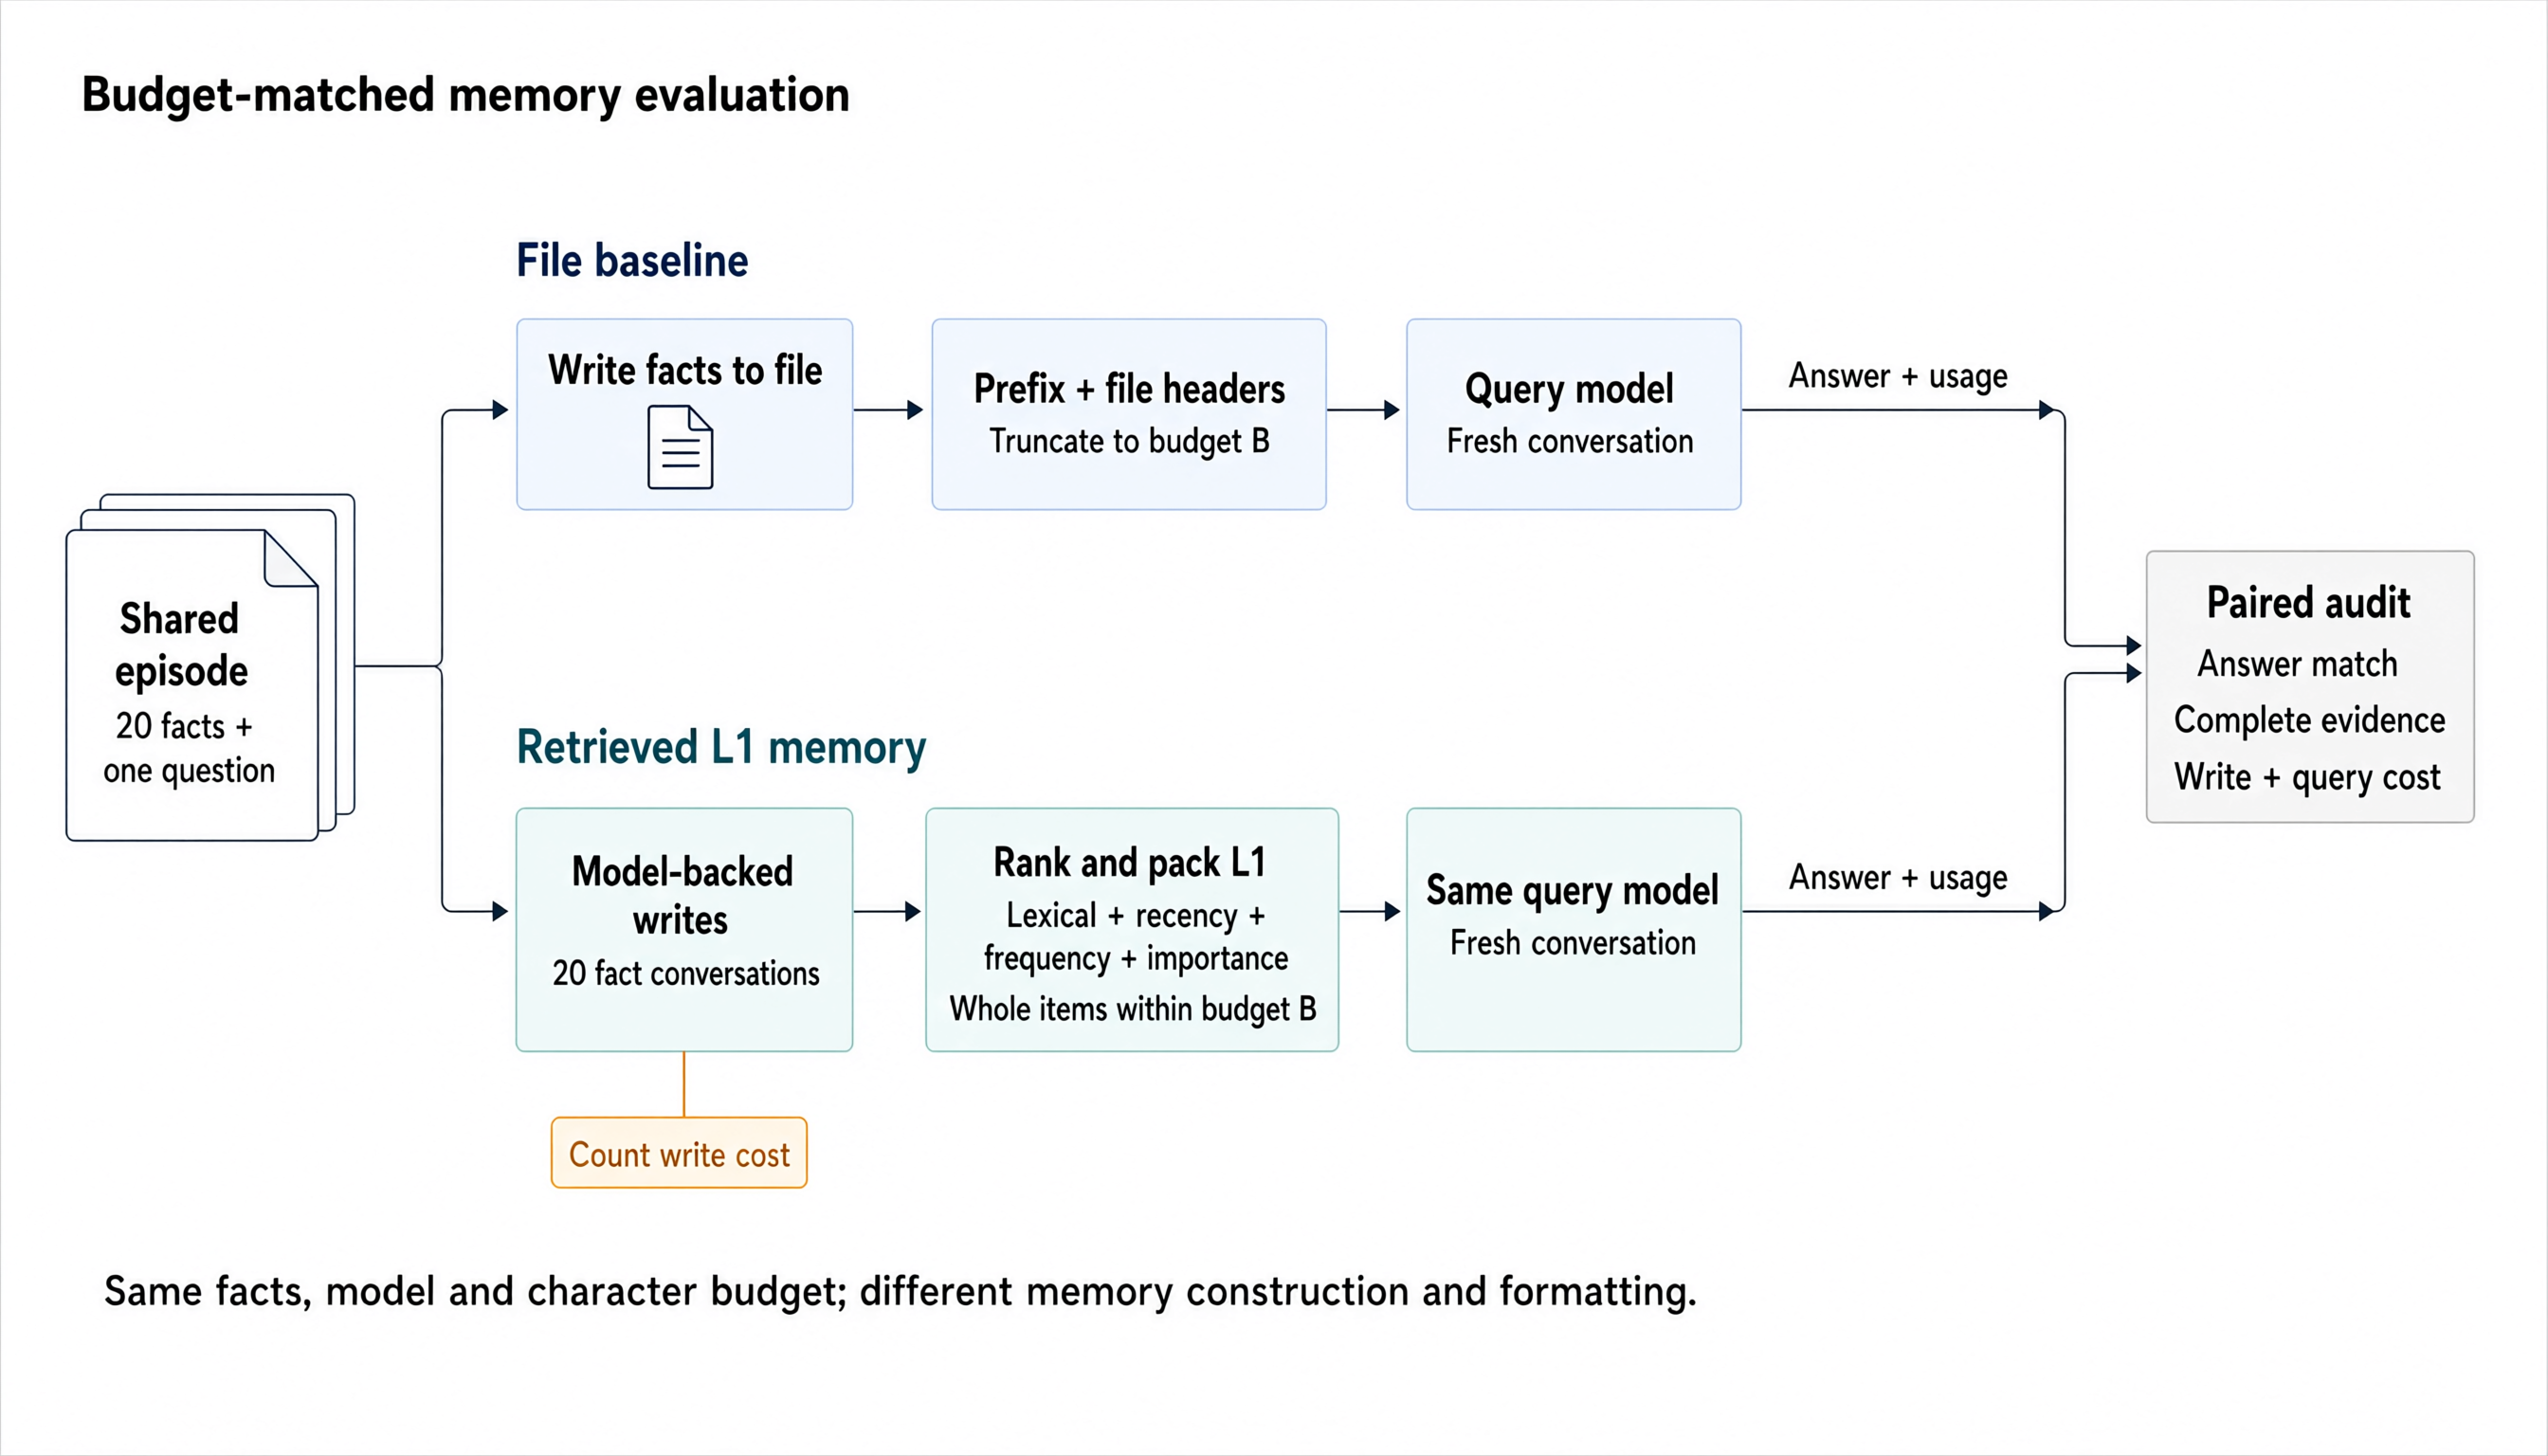
\includegraphics[width=\linewidth]{figures/methodology.png}
\caption{Budget-matched evaluation of two operational memory paths. The retrieved arm
incurs model-backed write cost before its isolated query. Equal character caps include
each arm's own formatting overhead. This schematic illustrates the audited implementation;
it is not an experimental result.}
\label{fig:methodology}\end{figure}
\subsection{Frozen Memory and Matched Token Packing}

\label{sec:method_baseline}

The baseline selectors operate on a frozen single-layer bank: complete source histories retained in their original form, segmented losslessly into turn segments bounded by a pinned Qwen3 BPE tokenizer. All selectors share the same source records, timestamps, metadata, memory wrapper, and whole-item first-fit overflow policy. The prefix selector uses bank order with no scoring. The recency selector keeps only the temporal decay term. The Jaccard selector keeps only lexical overlap over lowercased alphanumeric token sets. The deployed hybrid combines all four terms with fixed weights: lexical Jaccard overlap, temporal decay, bounded log-frequency, and heuristic importance. The hybrid\_no\_time ablation sets the temporal weight to zero and renormalizes remaining weights so lexical overlap retains proportional dominance. BM25 uses a standard probabilistic lexical score with positive inverse document frequency. The primary comparison is BM25 against the deployed hybrid.

The controlled comparison holds all variables fixed across arms: question identifiers, answering model and version, decoding settings, system prompt, canonical memory items, memory wrapper, tokenizer, packing policy, and write path. Only the selector scoring function changes. Frequency is held at a fixed value and importance at a fixed value across all selectors so that hybrid\_no\_time and Jaccard coincide as a sanity equivalence check, confirming that any remaining gap between the deployed hybrid and BM25 is attributable to the temporal term rather than to frequency or importance variation.

\subsection{Contrastive Tier-Based Lexical Selection (CTLS)}

\label{sec:method_ctls}

CTLS (Contrastive Tier-Based Lexical Selection) is a novel selector that partitions candidates into a lexically relevant tier (Jaccard overlap strictly positive) and a lexically absent tier (Jaccard overlap equal to zero) before applying any temporal scoring. Within the relevant tier, candidates are ranked by the full hybrid score so temporal decay and frequency serve as tiebreakers among genuinely relevant items. Within the absent tier, recency plus importance provides fallback ordering. Packing draws from the relevant tier first in descending score order, then from the absent tier in descending recency order, using the same whole-item first-fit policy as all other selectors. \citep{ref_959d6858d034c6e1}

The Non-Dominance Property follows directly from the tier partition. For any candidate with positive overlap and any candidate with zero overlap, CTLS places the positive-overlap item in the relevant tier and the zero-overlap item in the absent tier. Since packing exhausts the relevant tier entirely before inserting any absent-tier item, the relevant item is always considered for inclusion first, regardless of temporal decay, frequency, importance, or any weight values. No assignment of weights to temporal, frequency, or importance terms can cause an absent-tier item to displace a relevant-tier item. This eliminates temporal dominance by construction. CTLS requires no model calls, no embedding model, and no learned parameters. It is a zero-cost selector substitution compatible with the existing write path, packing policy, and memory wrapper. \citep{ref_ab2c226739f2f52a}

The relationship between CTLS and hybrid\_no\_time clarifies within-tier temporal ordering. hybrid\_no\_time discards temporal information entirely by setting the temporal weight to zero globally. CTLS preserves temporal decay as a within-tier tiebreaker: for two relevant-tier candidates with identical Jaccard scores, the temporal decay term breaks the tie. For queries where every candidate has positive overlap, CTLS and hybrid\_no\_time produce identical rankings when non-temporal terms are also equal, but CTLS retains recency information for cases where they differ. For mixed-tier queries -- the typical case for short questions against long conversational segments -- CTLS provably outperforms hybrid\_no\_time by guaranteeing relevant-tier priority. The hybrid\_no\_time empirical result is therefore a conservative lower bound on the improvement from CTLS.

\subsection{Repeated Real Agent Evaluation and Ablation Design}

\label{sec:method_protocol}

Each memory episode has its own fact set and fresh agent instances. The frozen bank design holds source records, timestamps, metadata, and segment content fixed across all selectors; write tokens are zero and construction cost is identical across every arm. The formal question uses a new conversation ID so that no seeding dialogue leaks into the query context. The runner verifies isolated query history and confirms actual memory injection before scoring. \citep{ref_ab2c226739f2f52a}

Evidence recall requires the complete annotated turn to appear in the delivered context; evidence-session recall requires any segment from the annotated session to be selected. Three answering calls per memory episode are averaged before stratified cluster bootstrap inference with Holm correction across all prespecified comparisons. The pinned original LongMemEval task-specific grading prompts are evaluated with a fixed primary judge model; strict yes/no parsing and arm-blind response keys replace substring grading. A second fixed model audits a deterministic sample. The evaluation adapts the stratified extraction paradigm of LongMemEval; the resulting subset is not an official benchmark score. Blinded human adjudication of model disagreements remains an open task before final paper submission.

\FloatBarrier

\subsection{Budget and cost formalization}
Let $q$ be a question, $M$ its episode memory, and $B$ the cap on the entire
injected memory section, including headings and metadata. The baseline constructs
a file-derived section and keeps its prefix. The retrieved arm scores stored
exchanges, takes at most $k=10$ candidates, and greedily appends complete formatted
items that fit. An over-budget item is skipped rather than partially appended;
later smaller items can still be considered. Thus equal $B$ does not imply equal
usable fact content or identical prompt formatting.
\begin{equation}
  s(q,m)=0.4J(T(q),T(m))+0.3\,2^{-a(m)/h}
       +0.2\min\!\left\{\frac{\log(1+f(m))}{\log(101)},1\right\}+0.1I(m),
  \label{eq:ranking}
\end{equation}
where $T$ lowercases text and keeps alphanumeric/underscore word tokens longer
than one character; $J(A,C)=|A\cap C|/|A\cup C|$ (zero for an empty set);
$a(m)$ is age in seconds; $h=86400$ is the decay half-life; $f(m)$ is the recorded
access count; and $I(m)$ is a bounded heuristic importance score. These are the
implementation's default weights, not learned or tuned coefficients. No embedding
model is invoked. L1 holds at most 20 exchanges with a one-hour time-to-live;
individual displayed exchanges are capped at 500 characters before packing.

The cost estimand includes initialization through model-backed memory writes:
\begin{equation}
 C_g=\frac{\sum_{r\in\mathcal{Q}_g}u_r+
                 \sum_{w\in\mathcal{W}_g}u_w}{N_{\rm valid}},\qquad
 L_g=\frac{\sum_{r\in\mathcal{Q}_g}t_r+
                 \sum_{w\in\mathcal{W}_g}t_w}{N_{\rm valid}}.
 \label{eq:accounting}
\end{equation}
Here $u$ and $t$ denote recorded token usage and elapsed time, respectively;
$\mathcal Q_g$ and $\mathcal W_g$ include all recorded query and write attempts.
The denominator counts valid matched question pairs. These timing sums exclude
unrecorded process initialization and are not a full application wall-clock time.
Missing usage remains unknown rather than zero.

For each valid pair, let $y_{g,i}$ indicate an accepted-answer substring match
and $e_{g,i}$ indicate that the complete target fact survived in the injected text:
\begin{equation}
 A_g=\frac{1}{N}\sum_i y_{g,i},\qquad
 R_g=\frac{1}{N}\sum_i e_{g,i},\qquad
 \Delta A=A_{\rm retrieved}-A_{\rm file}.
 \label{eq:metrics}
\end{equation}
The two indicators differ: a truncated fact can contain a sufficient answer span.
Wilson intervals describe finite-question uncertainty only. They do not estimate
model-run variability, correct the selected slice's bias, or establish significance.

\begin{table}[htbp]
\centering\small
\caption{Audited execution protocol. No component ablation or weight tuning is claimed.}
\label{tab:protocol}
\begin{tabular}{p{0.25\linewidth}p{0.66\linewidth}}\toprule
Step & Operation \\\midrule
Prepare & Create fresh isolated agents; give both arms the same fact episode. \\
Construct & Write the baseline file; seed retrieved L1 through separate fact conversations. \\
Query & Use a fresh conversation, no tools, one model iteration, and the assigned section budget. \\
Audit & Check actual prompt injection and isolated history before accepting a pair. \\
Aggregate & Match question IDs; count writes once per run; preserve excluded attempts in costs. \\
\bottomrule\end{tabular}\end{table}

\FloatBarrier
